\clearpage
\phantomsection
%\addcontentsline{toc}{chapter}{مقدمات}
\chapter{روش پیشنهادی}
\markboth{روش پیشنهادی}{عنوان فصل}
\section{آماده سازی داده ورودی}


مجموعه داده‌های MNIST\LTRfootnote{\lr{Modified National Institute of Standards and Technology database
}} و CIFAR-10 \LTRfootnote{\lr{Canadian Institute For Advanced Research}}‌ دو مجموعه داده معروف و پرکاربرد در حوزه تشخیص الگو هستند که به عنوان محیط‌های آزمایشی برای بسیاری از مدل‌ها و الگوریتم‌های یادگیری عمیق استفاده می‌شوند.

\subsection{ مجموعه داده MNIST}



این مجموعه داده شامل تصاویر دست‌نویسی از ارقام از ۰ تا ۹ است که به صورت ۲۸در۲۸ پیکسل و به صورت خاکستری نمایش داده می‌شوند. مجموعه داده MNIST به عنوان یک مجموعه آموزشی کلاسیک در تشخیص ارقام مورد استفاده قرار می‌گیرد و بسیاری از مدل‌های یادگیری عمیق از جمله شبکه‌های عصبی پیچشی  \LTRfootnote{\lr{ Convolutional neural network}}و  شبکه‌های عصبی بازگشتی {\large {\normalsize {\large \LTRfootnote{\lr{Recurrent neural network}}}}} بر روی آن آموزش می‌بینند. در این پروژه از این مجموعه داده برای آزمون میزان یادگیری خودنظارتی در شبکه عصبی اسپایکی استفاده شده است. در شکل  \ref{fig:data1}یک نمونه از مجموعه داده MNIST نشان داده شده است.

\begin{minipage}{\linewidth}
	\centering
	\includegraphics[width=10cm]{mnist.png}
	\captionsetup{font=small} % Adjust the font size of the caption
	\captionof{figure}{نمونه مجموعه داده MNIST}
	\label{fig:data1}
\end{minipage}

\subsection{ مجموعه داده CIFAR10}


مجموعه داده CIFAR10 شامل تصاویر رنگی از ده کلاس مختلف از اشیاء مختلف است. هر تصویر از این مجموعه داده ابعادی به اندازه ۳۲در۳۲ پیکسل و سه کانال رنگی (قرمز، سبز، آبی) دارد. این مجموعه داده به عنوان یک مجموعه آموزشی و ارزیابی محبوب در حوزه تشخیص الگو، تصویربرداری، و بینایی ماشین استفاده می‌شود. شبکه‌های عصبی پیچشی به خوبی برای طبقه‌بندی تصاویر در این مجموعه داده مورد استفاده قرار می‌گیرند . در این پروژه از این مجموعه داده به عنوان داده مورد تایید  برای سنجش کارآیی مدل ساخته شده با شبکه عصبی اسپایکی‌ استفاده می‌شود. در شکل \ref{fig:data2} یک نمونه از مجموعه داده CIFAR10 قابل مشاهده است.



\begin{minipage}{\linewidth}
	\centering
	\includegraphics[width=10cm]{cifar.png}
	\captionsetup{font=small} % Adjust the font size of the caption
	\captionof{figure}{نمونه مجموعه داده CIFAR10}
	\label{fig:data2}
\end{minipage}


این دو مجموعه داده از مجموعه داده‌های کلاسیک برای آموزش و ارزیابی مدل‌های یادگیری عمیق به شمار می‌آیند و با توجه به سادگی و قدرت تشخیصی‌شان، همچنان در مطالعات بسیاری از پژوهش‌های مرتبط با هوش مصنوعی و یادگیری ماشین مورد استفاده قرار می‌گیرند.

\subsection{افزایش داده}
برای استفاده از داده‌های مجموعه‌های MNIST و CIFAR10 در یادگیری خودنظارتی، افزایش حجم داده‌ها از اهمیت بسیاری برخوردار است. با اعمال تکنیک‌های مختلف افزایش حجم داده به داده‌های آموزشی، می‌توان تنوع بیشتری ایجاد کرد و عملکرد مدل‌ها را بهبود بخشید.

۱. چرخش\LTRfootnote{\lr{Rotation}} : 

با اعمال چرخش‌های مختلف به تصاویر، امکان ایجاد تصاویری با زوایای مختلف به وجود می‌آید. این تغییرات می‌تواند به مدل‌ها کمک کند تا به الگوها و تفاوت‌هایی که در زوایای مختلف وجود دارد، حساس‌تر شوند.

۲. برش \LTRfootnote{\lr{Crop}}:

 با برش بخش‌های تصاویر اصلی، می‌توان تصاویر جدید با ابعاد مختلف و محتواهای مختلف ایجاد کرد. این تغییرات به افزایش تنوع داده‌ها کمک می‌کند و می‌تواند اثرات مثبتی در یادگیری مدل‌ها داشته باشد.

۳. مات \LTRfootnote{\lr{Gaussian Blur}} :

 اعمال اثر مات به تصاویر می‌تواند جزئیات غیرضروری را حذف کند و برای مدل‌ها کار کردن با داده‌های نویزی را آموزش دهد. این تغییرات می‌تواند مدل‌ها را به صورت مستقل از تفاوت‌های جزئی در داده‌ها آموزش دهد.

۴. وارونه \LTRfootnote{\lr{Flip}} :

انعکاس تصاویر از روش‌های ساده و موثر برای افزایش حجم داده‌هاست. با اعمال این تغییر، تصاویر جدید با جهت‌های مختلف ایجاد می‌شوند که به مدل‌ها کمک می‌کند تا به الگوها و تفاوت‌های جهتی حساس‌تر شوند.

با اعمال این تغییرات به داده‌های MNIST و CIFAR10، می‌توان تعداد زیادی داده‌آموزشی جدید ایجاد کرد و مدل‌ها را با داده‌های متنوعی آموزش داد. این تنوع می‌تواند به افزایش دقت و کارایی مدل‌ها در مراحل بعدی یادگیری کمک کند و عملکرد آن‌ها را بهبود بخشد. با استفاده از داده‌های افزایش‌یافته, می‌توان به بهبود عملکرد یادگیری خودنظارتی بر روی شبکه‌های عصبی اسپایکی با اجرای الگوریتم‌های پیچیده‌تری در مراحل بعدی پرداخت. در این پروژه با استفاده از روش‌های مختلف افزودن داده روند یادگیری خودنظارتی شبکه عصبی اسپایکی را مورد بررسی قرار دادیم. در شکل\ref{fig:data4}  پیاده سازی روش‌های مختلف افزایش داده  بر روی داده‌های MNIST  و  CIFAR10 قابل مشاهده است.

\begin{minipage}{\linewidth}
	\centering
	\includegraphics[width=10cm]{mnist2.png}
	%\captionof{figure}{نمونه مجموعه داده MNIST}
	\label{fig:data3}
\end{minipage}

\begin{minipage}{\linewidth}
	\centering
	\includegraphics[width=10cm]{cifar2.png}
	\captionsetup{font=small} % Adjust the font size of the caption
	\captionof{figure}{  روش های افزودن داده . به ترتیب روش های مات, چرخش , وارون افقی و برش پیاده‌سازی شده‌است. }
	\label{fig:data4}
\end{minipage}



\section{ساخت معماری شبکه}

 در ساخت شبکه عصبی اسپایکی برای مدلسازی نورون نشت کننده و ادغام آتش از پکیج snntorch \LTRfootnote{\lr{https://snntorch.readthedocs.io/en/latest/index.html}} استفاده شده و  پیاده سازی اتصالات بین نورون ها به وسیله pytorch انجام شده است.
 هر نورون در مدل نورونی snntorch.leaky یک پارامتر به عنوان جریان و یک پارامتر به عنوان پتانسیل گام زمانی قبلی دریافت می‌کند و دو لیست با عنوان‌های اسپایک تولید شده توسط نورون(اگر پتانسیل از آستانه عبور کند برابر با یک و در غیر این صورت برابر با صفر خواهد بود.) و پتانسیل گام زمانی فعلی نورون را به عنوان خروجی می‌دهد. 
 \citep{eshraghian2021training}
 
 با توجه به اینکه مفهوم زمان در شبکه‌های عصبی اسپایکی مورد توجه است و داده‌ها در طول زمان به صورت جریان ثابت وارد شبکه شده و فرآیند تغییر پتانسیل و تولید اسپایک نیز در طول زمان اتفاق می افتد, خروجی مدل نورونی یک بعد زمان نیز دارد و داده‌ها که به صورت فریم‌های عکس در قالب جریان به نورون‌ها وارد می‌شوند در طول چند گام زمانی چندین بار وارد شبکه شده و تغییرات پتانسیل و گسیل اسپایک از نورون در گام‌های زمانی ضبط می‌شود.
 ساختار خروجی نورون‌ها به صورت :
\[
\left[ \text{step time} \times \text{ size batch} \times \text{ dimension feature} \right]
\]
 
 خواهد بود. در فرایند آموزش شبکه تابع هزینه را برای خروجی هر یک از نورون‌ها در تمام گام‌های زمانی محاسبه کرده و در نهایت مجموع آن را به عنوان مقدار هزینه در نظر می‌گیریم و سعی در کمینه کردن آن داریم.
 
  برای اتصالات بین نورون‌ها از لایه‌های پیچشی و همچنین از لایه‌های کاملا متصل استفاده کرده‌ایم. با توجه به اینکه معماری‌های شبکه‌های عصبی پیچشی برای یادگیری خودنظارتی مناسب هستند معماری شبکه عصبی اسپایکی را با الهام از شبکه‌های پیچشی پیاده‌سازی کرده و مدل نورونی را نشت کننده و ادغام آتش قرار دادیم.

در ادامه به توضیح بیشتر معماری مدل نورونی و اتصال لایه‌ها در شبکه می‌پردازیم :

لایه‌های پیچشی \LTRfootnote{\lr{Convolutional layers}}:

شبکه با یک سری لایه‌ پیچشی شروع می‌شود. این لایه‌ها عملیات پیچش دو بعدی را روی داده‌های ورودی انجام می دهند. این لایه‌ها به گونه‌ای طراحی شده‌اند که با اعمال مجموعه‌ای از فیلترهای قابل یادگیری (هسته‌ها\LTRfootnote{\lr{Kernel}}) ویژگی‌ها را در تصاویر ورودی ثبت کنند. این فیلترها روی تصویر می لغزند و نقشه‌های ویژگی را تولید می کنند که جنبه‌های مختلف ورودی را برجسته می کند.
\citep{o2015introduction}

لایه‌های عصبی نشت کننده و ادغام آتش :(LIF)

بعد از هر لایه پیچشی، یک لایه نورون نشت‌کننده و ادغام و آتش (LIF) مربوطه اعمال می شود. این لایه‌ها مدل نورون LIF را پیاده‌سازی می‌کنند. نورون‌های LIF رفتار نورون‌های واقعی را با ادغام اسپایک‌های ورودی در طول زمان شبیه سازی می کنند. اگر پتانسیل غشای یکپارچه از یک آستانه خاص فراتر رود، نورون یک اسپایک خروجی ساطع می کند. مدل LIF یک پارامتر نشتی را نیز معرفی می‌کند که کاهش تدریجی پتانسیل غشا را در طول زمان نشان می‌دهد.


حداکثر ادغام \LTRfootnote{\lr{Max-pooling}}:

در سراسر شبکه، لایه‌های حداکثر ادغام پس از لایه‌های پیچشی و LIF اعمال می‌شوند. این لایه‌ها نقشه‌های ویژگی به‌دست‌آمده از لایه‌های قبلی را پایین می‌آورد و ابعاد فضایی آن‌ها را کاهش می‌دهد. این عملیات به استخراج ویژگی‌های کلیدی از داده‌ها کمک می‌کند و در عین حال پیچیدگی محاسباتی را کاهش می‌دهد.


لایه‌های کاملا متصل\LTRfootnote{\lr{Fully connected}}:

در انتهای شبکه، از لایه‌های کاملاً متصل برای کاهش بعد نقشه‌های ویژگی به‌دست‌آمده از لایه‌های قبلی و تبدیل آن‌ها به یک بردار تک بعدی استفاده می‌شود. این لایه‌ها تبدیل‌های خطی روی داده‌ها انجام می‌دهند. لایه‌های نورون LIF مشابه لایه‌های قبلی بعد از لایه‌های کاملا متصل نیز اعمال می‌شوند.

در شکل  \ref{fig:arc} یک نمونه از نوع اتصالات لایه‌ها در شبکه نشان داده‌شده است. لازم به ذکر است لایه‌های نورونی اسپایکی در بین هریک از اتصالات شبکه قرار گرفته و خروجی اسپایکی نورون‌ها به وسیله اتصالات در شبکه فرآیند یادگیری را طی می‌کنند.

\begin{minipage}{\linewidth}
	\centering
	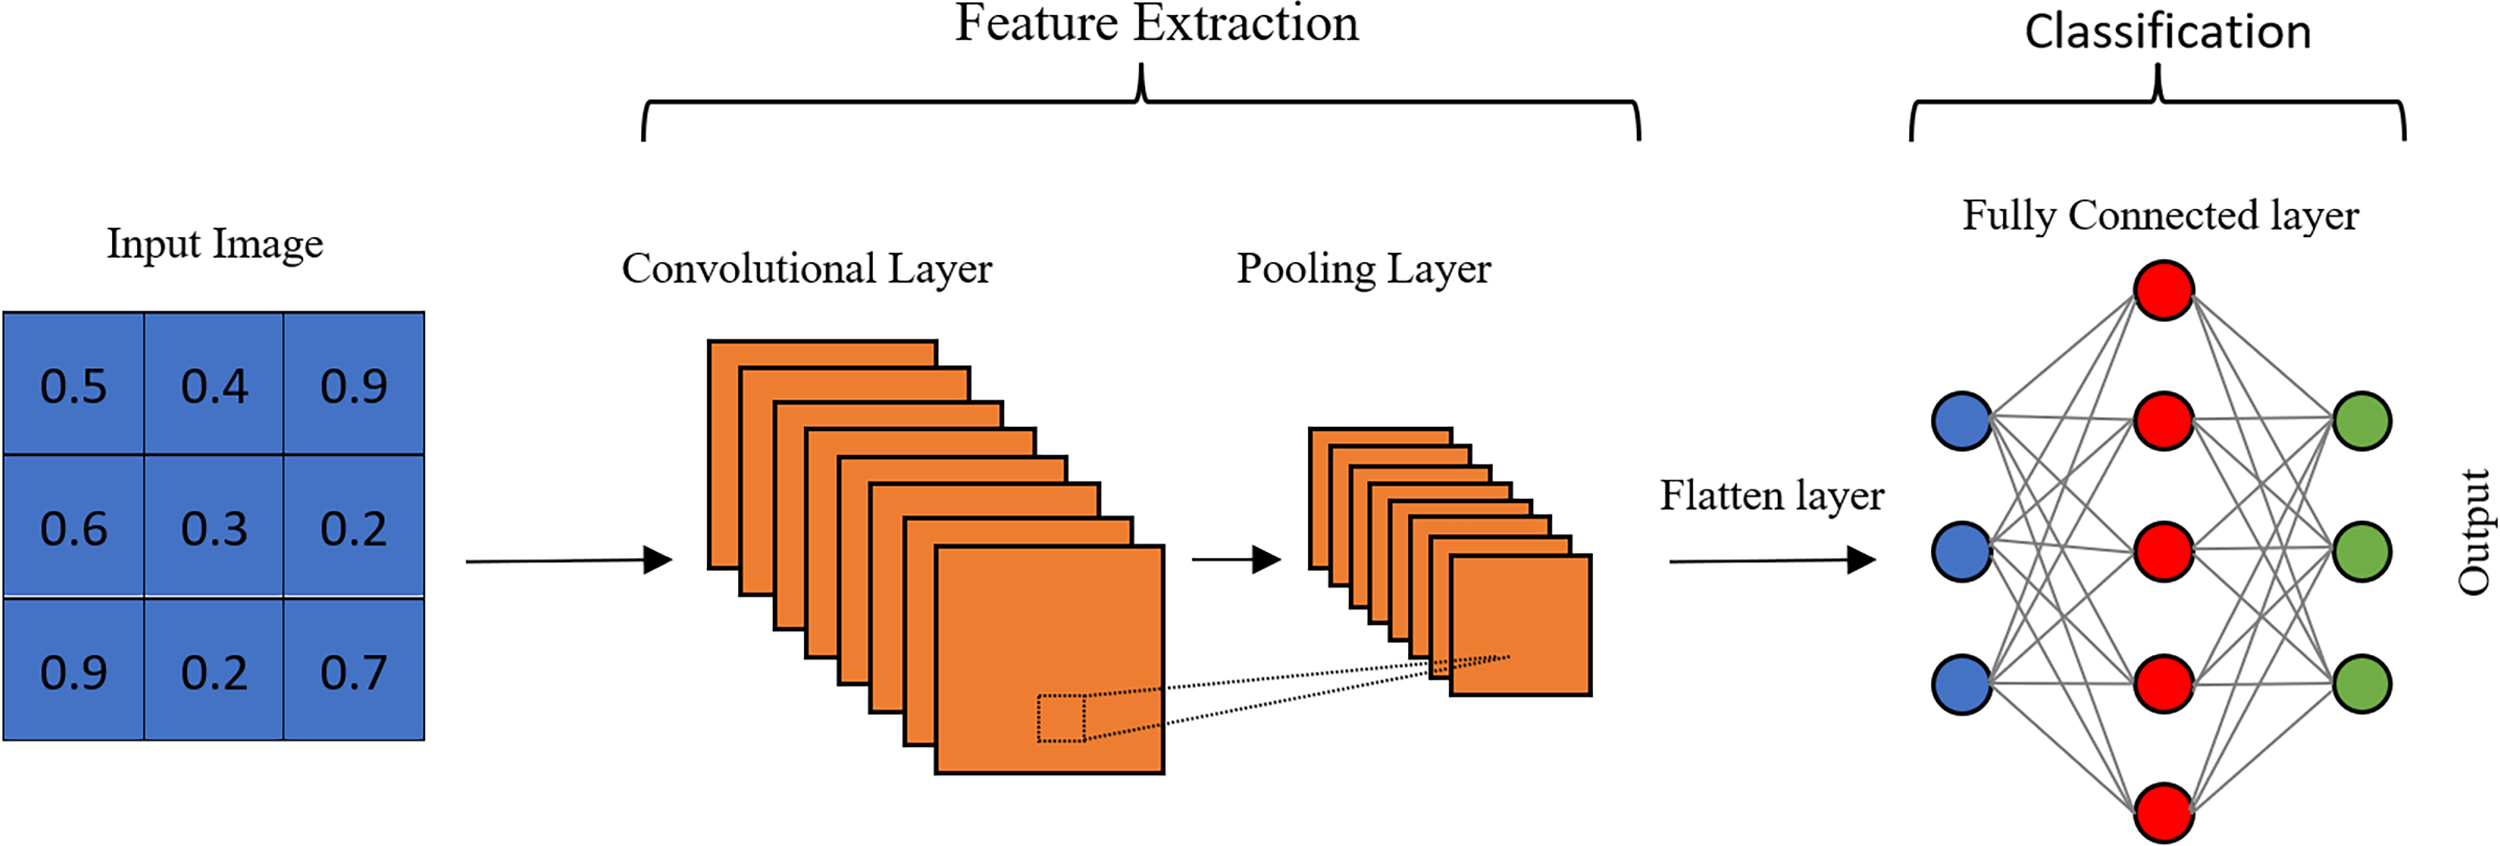
\includegraphics[width=10cm]{arc.png}
	\captionsetup{font=small} % Adjust the font size of the caption
	\captionof{figure}{شکل کلی اتصالات لایه‌های پیچشی, حداکثر ادغام و کاملا متصل در معماری شبکه ساخته شده. لایه ‌های پیچشی و حداکثر ادغام وظیفه اس تخراج ویژگی و لایه‌های ماکلا متصل وظیفه دسته‌بندی را به عهده دارند. نورون‌ها با مدل نورونی نشت‌کننده و ادغام آتش در بین تمام لایه‌های اتصال پیاده‌سازی شده‌اند. }
	\label{fig:arc}
\end{minipage}





تابع رو به جلو \LTRfootnote{\lr{Forward function}}:

در مسیر یادگیری رو به جلو، داده‌های ورودی از طریق لایه‌های پیچشی، حداکثر ادغام و کاملا متصل به صورت گام به گام پردازش می شوند. پتانسیل‌های غشایی نورون‌های LIF در طول مراحل زمانی به روز می‌شوند و اگر پتانسیل غشایی یک نورون از آستانه عبور کند، یک اسپایک خروجی ایجاد می‌شود. اسپایک‌های خروجی در چندین مرحله زمانی جمع‌آوری می‌شوند و به صورت دنباله‌ای از تانسورهای اسپایک بازگردانده می‌شوند.

به طور خلاصه، این شبکه عصبی اسپایکی از لایه‌های پیچشی برای استخراج ویژگی‌ها، لایه‌های نورون LIF برای شبیه‌سازی رفتار عصبی، لایه‌های حداکثر ادغام برای کاهش بعد نمونه‌برداری  و لایه‌های کاملاً متصل برای دسته‌بندی تشکیل شده است. 


در نهایت، با استفاده از لایه‌های پیچشی و مدل‌های نورونی اسپایکی، مدل عصبی می‌تواند ویژگی‌های مهم از داده‌های MNIST و CIFAR-10 استخراج کند و افزایش حجم داده با استفاده از تکنیک‌های گفته‌شده نیز می‌تواند بهبود قابل توجهی در یادگیری مدل ایجاد کند و دقت و عملکرد آن را افزایش دهد و همزمان نیز نیاز به داده برچسب‌دار را کاهش دهد.


\section{انتخاب الگوریتم خودنظارتی مناسب}


انتخاب روش SimCLR برای پیاده‌سازی بر روی شبکه عصبی اسپایکی نسبت به روش‌های خودنظارتی دیگر، دلایل متعددی دارد. از جمله مهم‌ترین دلایل این انتخاب، کارایی و اثربخشی روش SimCLR در یادگیری نمایش‌ها و استخراج ویژگی‌های معنادار از داده‌ها است. SimCLR از دو مرحله اصلی تشکیل شده است که شامل تولید نمونه‌های توسعه‌یافته و استفاده از تابع هدف مبتنی بر تفاوت نمونه‌ها می‌شود. این دو مرحله باعث می‌شوند که مدل با افزایش حجم داده‌ها و تلاش برای افزایش شباهت نمونه‌های مشابه و کاهش تفاوت نمونه‌های مختلف، ویژگی‌های با اهمیت و معنادار از داده‌ها استخراج کند.
در شکل \ref{fig:sim} روش کلی پیاده سازی این الگوریتم نشان داده شده است.

\begin{minipage}{\linewidth}
	\centering
	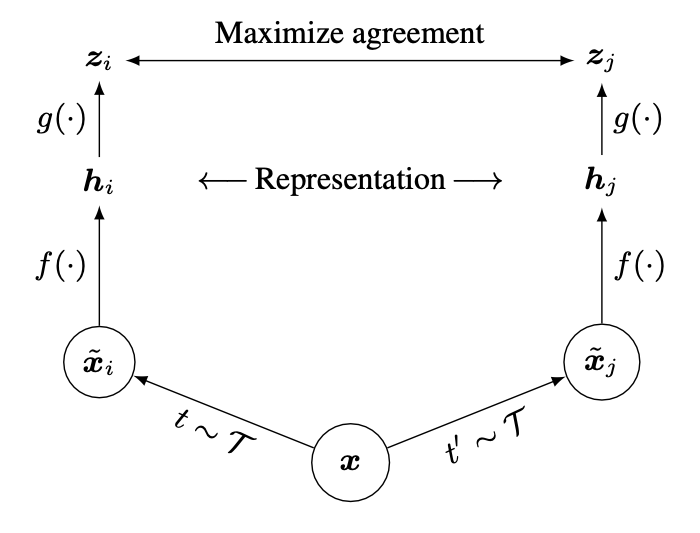
\includegraphics[width=8cm]{simf.png}
	\captionsetup{font=small} % Adjust the font size of the caption
	\captionof{figure}{الگوریتم simclr با کمینه کردن فاصله میان نمونه‌های افزوده شده از یک داده در فضای نمونه, نمایش‌های مناسب از داده بدون برچسب‌را تولید می‌کند.}
	\label{fig:sim}
\end{minipage}


به علاوه، SimCLR به عنوان یکی از روش‌های معتبر یادگیری خودنظارتی، به‌طور گسترده‌ای مورد آزمایش و ارزیابی قرار گرفته است و نتایج بسیار خوبی در استخراج ویژگی‌ها از داده‌ها و بهبود کارایی مدل‌های عصبی حاصل کرده است. این روش می‌تواند بر روی مجموعه‌های داده‌های کوچکتر نیز به‌کار گرفته شود و نیاز به برچسب‌گذاری داده‌ها ندارد .

با توجه به مزیت‌ها و نتایج امتحان‌شده روش SimCLR در حوزه‌های دیگر یادگیری خودنظارتی، انتخاب این روش برای استفاده در شبکه عصبی اسپایکی می‌تواند به عنوان یک انتخاب مناسب و ارزشمند محسوب شود که می‌تواند به بهبود کارایی و عملکرد کلی مدل بسیار کمک کند.







\section{انتخاب تابع هزینه}

در پیاده سازی الگوریتم simclr از تابع هزینه آنتروپی متقاطع با مقیاس دمایی نرمال شده استفاده می شود:


\begin{equation}
	\mathcal{L}_{\text{NTXent}} = -\frac{1}{N} \sum_{i=1}^{N} \log \frac{\exp(\text{sim}(z_i, z_{\text{pos}}) / \tau)}{\sum_{j=1}^{2N} \exp(\text{sim}(z_i, z_j) / \tau)}
\end{equation}

برای پیاده سازی این تابع هزینه با توجه به ساختار نمایش‌های ساخته شده توسط شبکه از کتابخانه pytorch metric learning استفاده کرده ایم. به این صورت که تابع دو نمونه افزوده شده از داده اصلی را به عنوان ورودی می‌گیرد و مقدار شباهت کسینوسی آن را محاسبه کرده و تقسیم بر مجموع همین مقدار برای تمام جفت‌های مثبت می‌کند و در نهایت لگاریتم این مقدار را ذخیره می‌کند.



\section{انتخاب بهینه‌ساز}

بهینه‌ساز یک عنصر کلیدی در فرآیند یادگیری ماشین و شبکه‌های عصبی است. به‌طور کلی، بهینه‌سازها ابزارهایی هستند که در فرآیند تغییر پارامترهای مدل با هدف کمینه کردن تابع هزینه یا خطا به‌کار می‌روند. این پارامترها به‌طور معمول وزن‌ها و بایاس‌های موجود در شبکه‌های عصبی و دیگر پارامترهای مدل یادگیری ماشین را شامل می‌شوند.

هدف اصلی بهینه‌سازها این است که پارامترها را به گونه‌ای تغییر دهند که تابع هزینه کمینه شود. این کار معمولاً با محاسبه گرادیان تابع هزینه نسبت به پارامترها آغاز می‌شود. گرادیان نشان دهنده جهت و شیب تابع در نقاط مختلف است و اطلاعاتی درباره روش تغییرات پارامترها را ارائه می‌دهد.

نوع بهینه‌سازی مورد استفاده می‌تواند تأثیر زیادی بر سرعت و کیفیت یادگیری داشته باشد. بهینه‌سازها ممکن است معیارهای مختلفی را در نظر بگیرند تا در جلوگیری از بیش‌برازش  \LTRfootnote{\lr{Overfitting}}مدل کمک کنند.

استفاده از بهینه‌ساز مناسب می‌تواند به تسریع فرآیند یادگیری، افزایش دقت مدل و جلوگیری از مشکلات مانند بیش‌برازش کمک کند. انتخاب بهینه‌ساز باید با توجه به مساله موردنظر، نوع داده‌ها و معماری مدل انجام شود.

بهینه‌ساز Adam یک روش پیشرفته و موثر در فرآیند یادگیری ماشین و شبکه‌های عصبی است. 
یکی از ویژگی‌های منحصر به فرد Adam، استفاده از نرخ یادگیری انطباقی است. این به معنای تنظیم خودکار نرخ یادگیری بر اساس ویژگی‌های داده‌ها و مساله است. این ویژگی باعث می‌شود Adam به طور خودکار با تغییرات متغیری در داده‌ها، به سرعت به نقاط بهینه همگرا شود.
Adam به طور معمول به سرعت به نقاط بهینه همگرا می‌شود و در مواجهه با داده‌های نویزی نیز خوب عمل می‌کند. از این رو، این بهینه‌ساز به‌طور گسترده در زمینه‌های مختلف یادگیری ماشین و شبکه‌های عصبی مورد استفاده قرار می‌گیرد.

در این پروژه برای پیاده سازی شبکه عصبی اسپایکی با روش یادگیری خودنظارتی از بهینه ساز Adam استفاده شده است. و با استفاده از کتابخانه pytorch پیاده سازی شده است.
\citep{kingma2014adam}

\section{الگوریتم نزدیک ترین همسایه(KNN) }

با توجه به اینکه به وسیله روش یادگیری خودنظارتی شبکه می‌آموزد نمایش هایی از داده اصلی تولید کند برای بررسی اینکه این نمایش های تولید شده چه میزان قابل اعتماد هستند و شبکه تا چه حد آموخته که نمایش مناسبی از داده تولید کند, الگوریتم نزدیک ترین همسایه را برای نمایش‌های تولید شده توسط شبکه پیاده سازی کرده و مشاهده می‌کنیم برای نمونه‌های تصادفی از نمایش‌های تولید شده از داده اصلی نزدیک ترین همسایه‌ها تا چه حد مشابه نمایش‌های تولید شده از داده اصلی هستند. معمولا در الگوریتم نزدیک ترین همسایه با توجه به اکثریت همسایه‌های نمونه که در واقع کمترین معیار فاصله از داده را در فضای نمونه دارند, خود داده اصلی در گروه اکثریت همسایه‌ها با همان برچسب قرار می‌گیرد اما در این پروژه استفاده از الگوریتم نزدیک ترین همسایه برای آزمایش نمایش‌های تولید شده توسط شبکه با الگوریتم یادگیری خودنظارتی است و نتایج آن صرفا برای این هدف مشاهده می‌شوند. در شکل  \ref{fig:knnn}عملکرد کلی این الگوریتم برای یافتن نزدیک ترین همسایه نشان داده شده است.
\citep{guo2003knn}


\begin{minipage}{\linewidth}
	\centering
	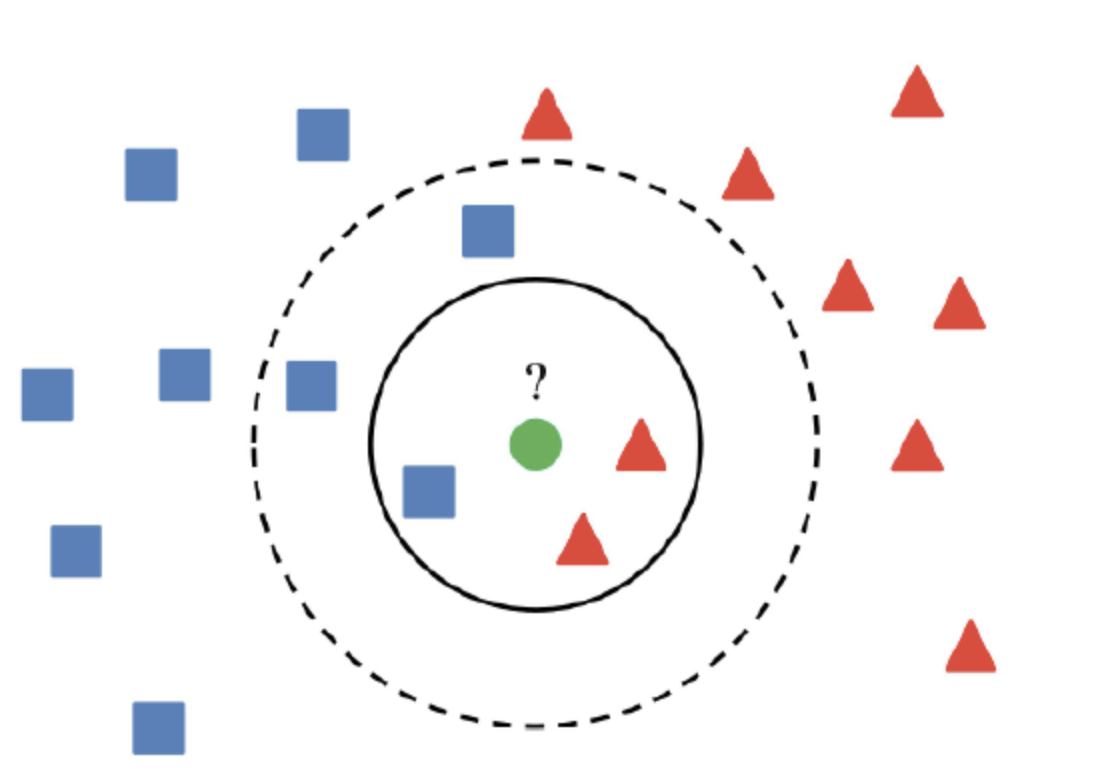
\includegraphics[width=8cm]{knn.png}
	\captionsetup{font=small} % Adjust the font size of the caption
	\captionsetup{font=small} % Adjust the font size of the caption
	\captionof{figure}{الگوریتم نزدیک ترین همسایه}
	\label{fig:knnn}
\end{minipage}


الگوریتم نزدیک‌ترین همسایه (KNN) یکی از الگوریتم‌های یادگیری ماشینی بدون نظارت است که برای دسته‌بندی و پیش‌بینی داده‌ها به کار می‌رود. اصول عمل این الگوریتم بسیار ساده است و بر مفهوم نزدیکی داده‌ها در فضای ویژگی‌ها بنا شده است.

راهکار الگوریتم KNN در پیدا کردن همسایه‌های نزدیک:

فرض کنید ما  مجموعه‌ای از داده‌ها را داریم و می‌خواهیم برای تعدادی نمونه تصادفی که به ما داده می‌شود، نزدیک‌ترین همسایه‌های آن را پیدا کنیم. راهکار الگوریتم KNN به این صورت است:

1. انتخاب تعداد همسایه (K):

ابتدا باید تعداد همسایه‌هایی که می‌خواهیم پیدا کنیم را انتخاب کنیم. این تعداد به عنوان K شناخته می‌شود.

2. محاسبه فواصل:

 برای هر داده ما باید فاصله‌ی آن با تمام داده‌های موجود در مجموعه‌داده را محاسبه کنیم. این فواصل معمولاً با استفاده از معیارهای مختلفی مانند فاصله اقلیدسی یا فاصله کسینوسی محاسبه می‌شوند.

3. انتخاب همسایه‌ها:

سپس تعداد همسایه‌ای که کمترین فواصل را با داده جدید دارند به عنوان همسایه‌های نزدیک انتخاب می‌شوند.
  و در نهایت نتیجه الگوریتم را بر روی نمایش های تولید شده توسط شبکه مشاهده و بررسی می‌کنیم.





\section{دسته‌بندی کننده}



در زمینه یادگیری خودنظارتی، وجود دسته‌بندی کننده \LTRfootnote{\lr{Classifier head}}یک جزء مهم است که برای ارزیابی کیفیت نمایش‌های آموخته‌شده استفاده می‌شود. این یک لایه شبکه عصبی اضافی است که به ویژگی‌های آموخته شده استخراج شده از شبکه  اصلی متصل است. هدف اصلی دسته‌بندی‌کننده، تبدیل نمایش‌های تولیده شده توسط شبکه به برچسب‌های کلاس یا سایر پیش‌بینی‌های مرتبط است که می‌تواند برای وظایف نظارت‌شده استفاده شود.

 دسته‌بندی کننده با استفاده از وظیفه خود نظارتی آموزش داده می شود. این به این معنی است که در طول مرحله آموزش خود‌‌نظارتی، سر دسته‌بندی کننده برای پیش‌بینی برخی ویژگی‌های خاص داده‌های ورودی که به روشی خاص تبدیل یا تقویت شده‌اند، آموزش داده می‌شود. این ویژگی می تواند چرخش، رنگ آمیزی و غیره باشد، بسته به روش خود نظارتی انتخاب شده اند. 
 ابتدا شبکه عصبی پیاده‌سازی شده نمایش‌ها را از داده تقویت شده تولید می‌کند و می آموزد فاصله نمایش های داده‌های یکسان و در یک دسته را بدون برچسب طی فرایند یادگیری خودنظارتی کمینه کند سپس از شبکه آموزش دیده برای به کار گیری در وظایفی مانند دسته بندی نظارت شده استفاده می‌شود. در این مرحله یک دسته بندی کننده که در این پروژه از یک لایه کاملا متصل استفاده می‌شود  بعد نمایش خروجی شبکه را به تعداد دسته‌های نهایی مورد نظر کاهش می‌دهد و از بردار خروجی برای وظایف نظارت‌شده استفاده ‌می‌کند.

به طور خلاصه،  دسته‌بندی کننده در یادگیری خود نظارتی به عنوان پلی بین وظیفه خود نظارت شده و وظایف نظارت‌شده  عمل می کند و به شبکه اجازه می دهد تا نمایش های معنی دار را از داده‌های بدون برچسب یاد بگیرد و سپس این نمایش‌ها را برای کارهای خاص تنظیم یا تطبیق دهد.

در این پروژه ابتدا شبکه با داده بدون برچسب با روش یادگیری خودنظارتی نمایش‌هایی از داده تولید می‌کند و در ادامه شبکه به علاوه  دسته‌بندی کننده با داده با حجم کم برچسب‌دار طی یک فرآیند یادگیری نظارت شده یک عملیات دسته بندی را انجام می‌دهد به این صورت که یک بار شبکه اصلی به عنوان یک ستون  \LTRfootnote{\lr{Backbone}}به  دسته‌بندی کننده متصل می‌شود و با نرخ یادگیری پایین بر روی داده برچسب‌دار با حجم کم آموزش ‌می‌بیند. و یک بار نیز وزن‌های شبکه آموزش دیده شده را ثابت نگه داشته و تنها  دسته‌بندی کننده آموزش می‌بیند و نتایج را مشاهده کرده و با یادگیری از ابتدا نظارت شده مقایسه می‌کنیم.

امید است فرایند یادگیری خودنظارتی در افزایش دقت شبکه در عملیات نهایی دسته بندی با داده برچسب دار با حجم کم موثر واقع شود. در نتیجه در انتهای فرآیند یادگیری شبکه , یک بار نیز همان شبکه را با حجم داده کم و از ابتدا نظارت شده آموزش می‌دهیم تا نتیجه هر دو روش را با هم مقایسه کرده و میزان تاثیر فرایند خودنظارتی را بررسی کنیم.

در شکل \ref{fig:class} یک نمونه از معماری شبکه در یادگیری خودنظارتی نمایش داده شده است که ابتدا یک افزایش داده پیاده‌سازی شده و سپس یک شبکه عصبی اسپایکی با لایه‌های پیچشی و حداکثر ادغام وظیفه تولید نمایش‌های داده را به عهده دارد و در نهایت نیز لایه کاملا متصل دسته‌بندی را روی نمایش‌های تولید شده اعمال کرده و تابع هزینه بر روی آن محاسبه می‌شود.




\begin{minipage}{\linewidth}
	\centering
	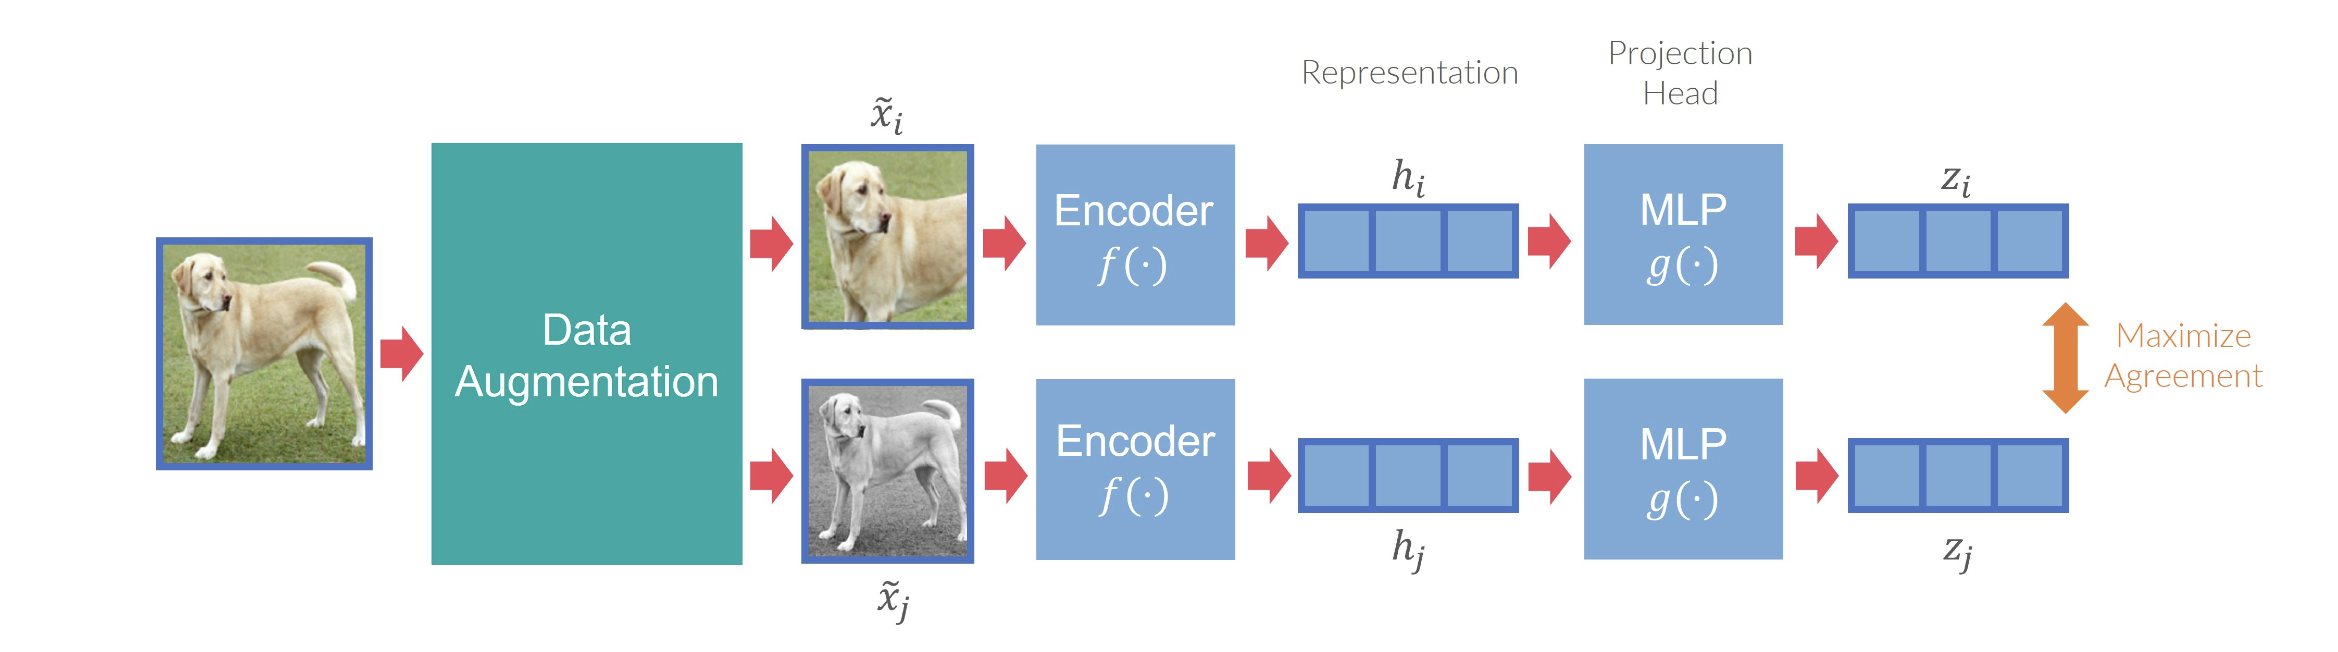
\includegraphics[width=12cm]{class.png}
	%\captionof{figure}{انتقال یادگیری در مقایسه در فرایند یادگیری خودنظارتی}
	\label{fig:class}
\end{minipage}

با توجه به توضیحات داده شده برای پیاده سازی و روش شناسی حل مساله در فصل بعد نتایج پیاده سازی را مشاهده و بررسی می‌کنیم.



